\section{Results}

\subsection{Baseline Overview}

The baseline evaluation includes 3,925 Imagenette validation images, with a top-1 accuracy of 87.18\% and a total source size of 97.81 MiB. ImageWoof includes 3,929 validation images, with a baseline accuracy of 88.27\% and a total source size of 96.71 MiB.

\subsection{Imagenette Results}

For Imagenette, JPEG q95 and q80 and WebP q95 produce outputs larger than the distributed source files, despite retaining accuracy close to the baseline. The first tested JPEG condition providing useful storage reduction is q60, which reduces total size by 11.2\% and changes accuracy by $-1.30$ percentage points. WebP q80 provides a similar size reduction of 12.9\% with a smaller observed accuracy change of $-0.84$ percentage points. At stronger compression levels, both codecs show progressively lower PSNR, SSIM, and classification accuracy.

\subsection{ImageWoof Results}

For ImageWoof, JPEG q95 and q80 and WebP q95 also increase the total file size. At approximately similar mild compression levels, JPEG q60 reduces storage by 10.6\% with an observed accuracy change of $-1.58$ percentage points, while WebP q80 reduces storage by 11.9\% with a smaller observed change of $-0.74$ percentage points. Accuracy degradation becomes more pronounced under aggressive compression: JPEG q10 changes accuracy by $-16.42$ percentage points, compared with $-10.66$ percentage points for WebP q10.

\begin{table}[!htbp]
    \centering
    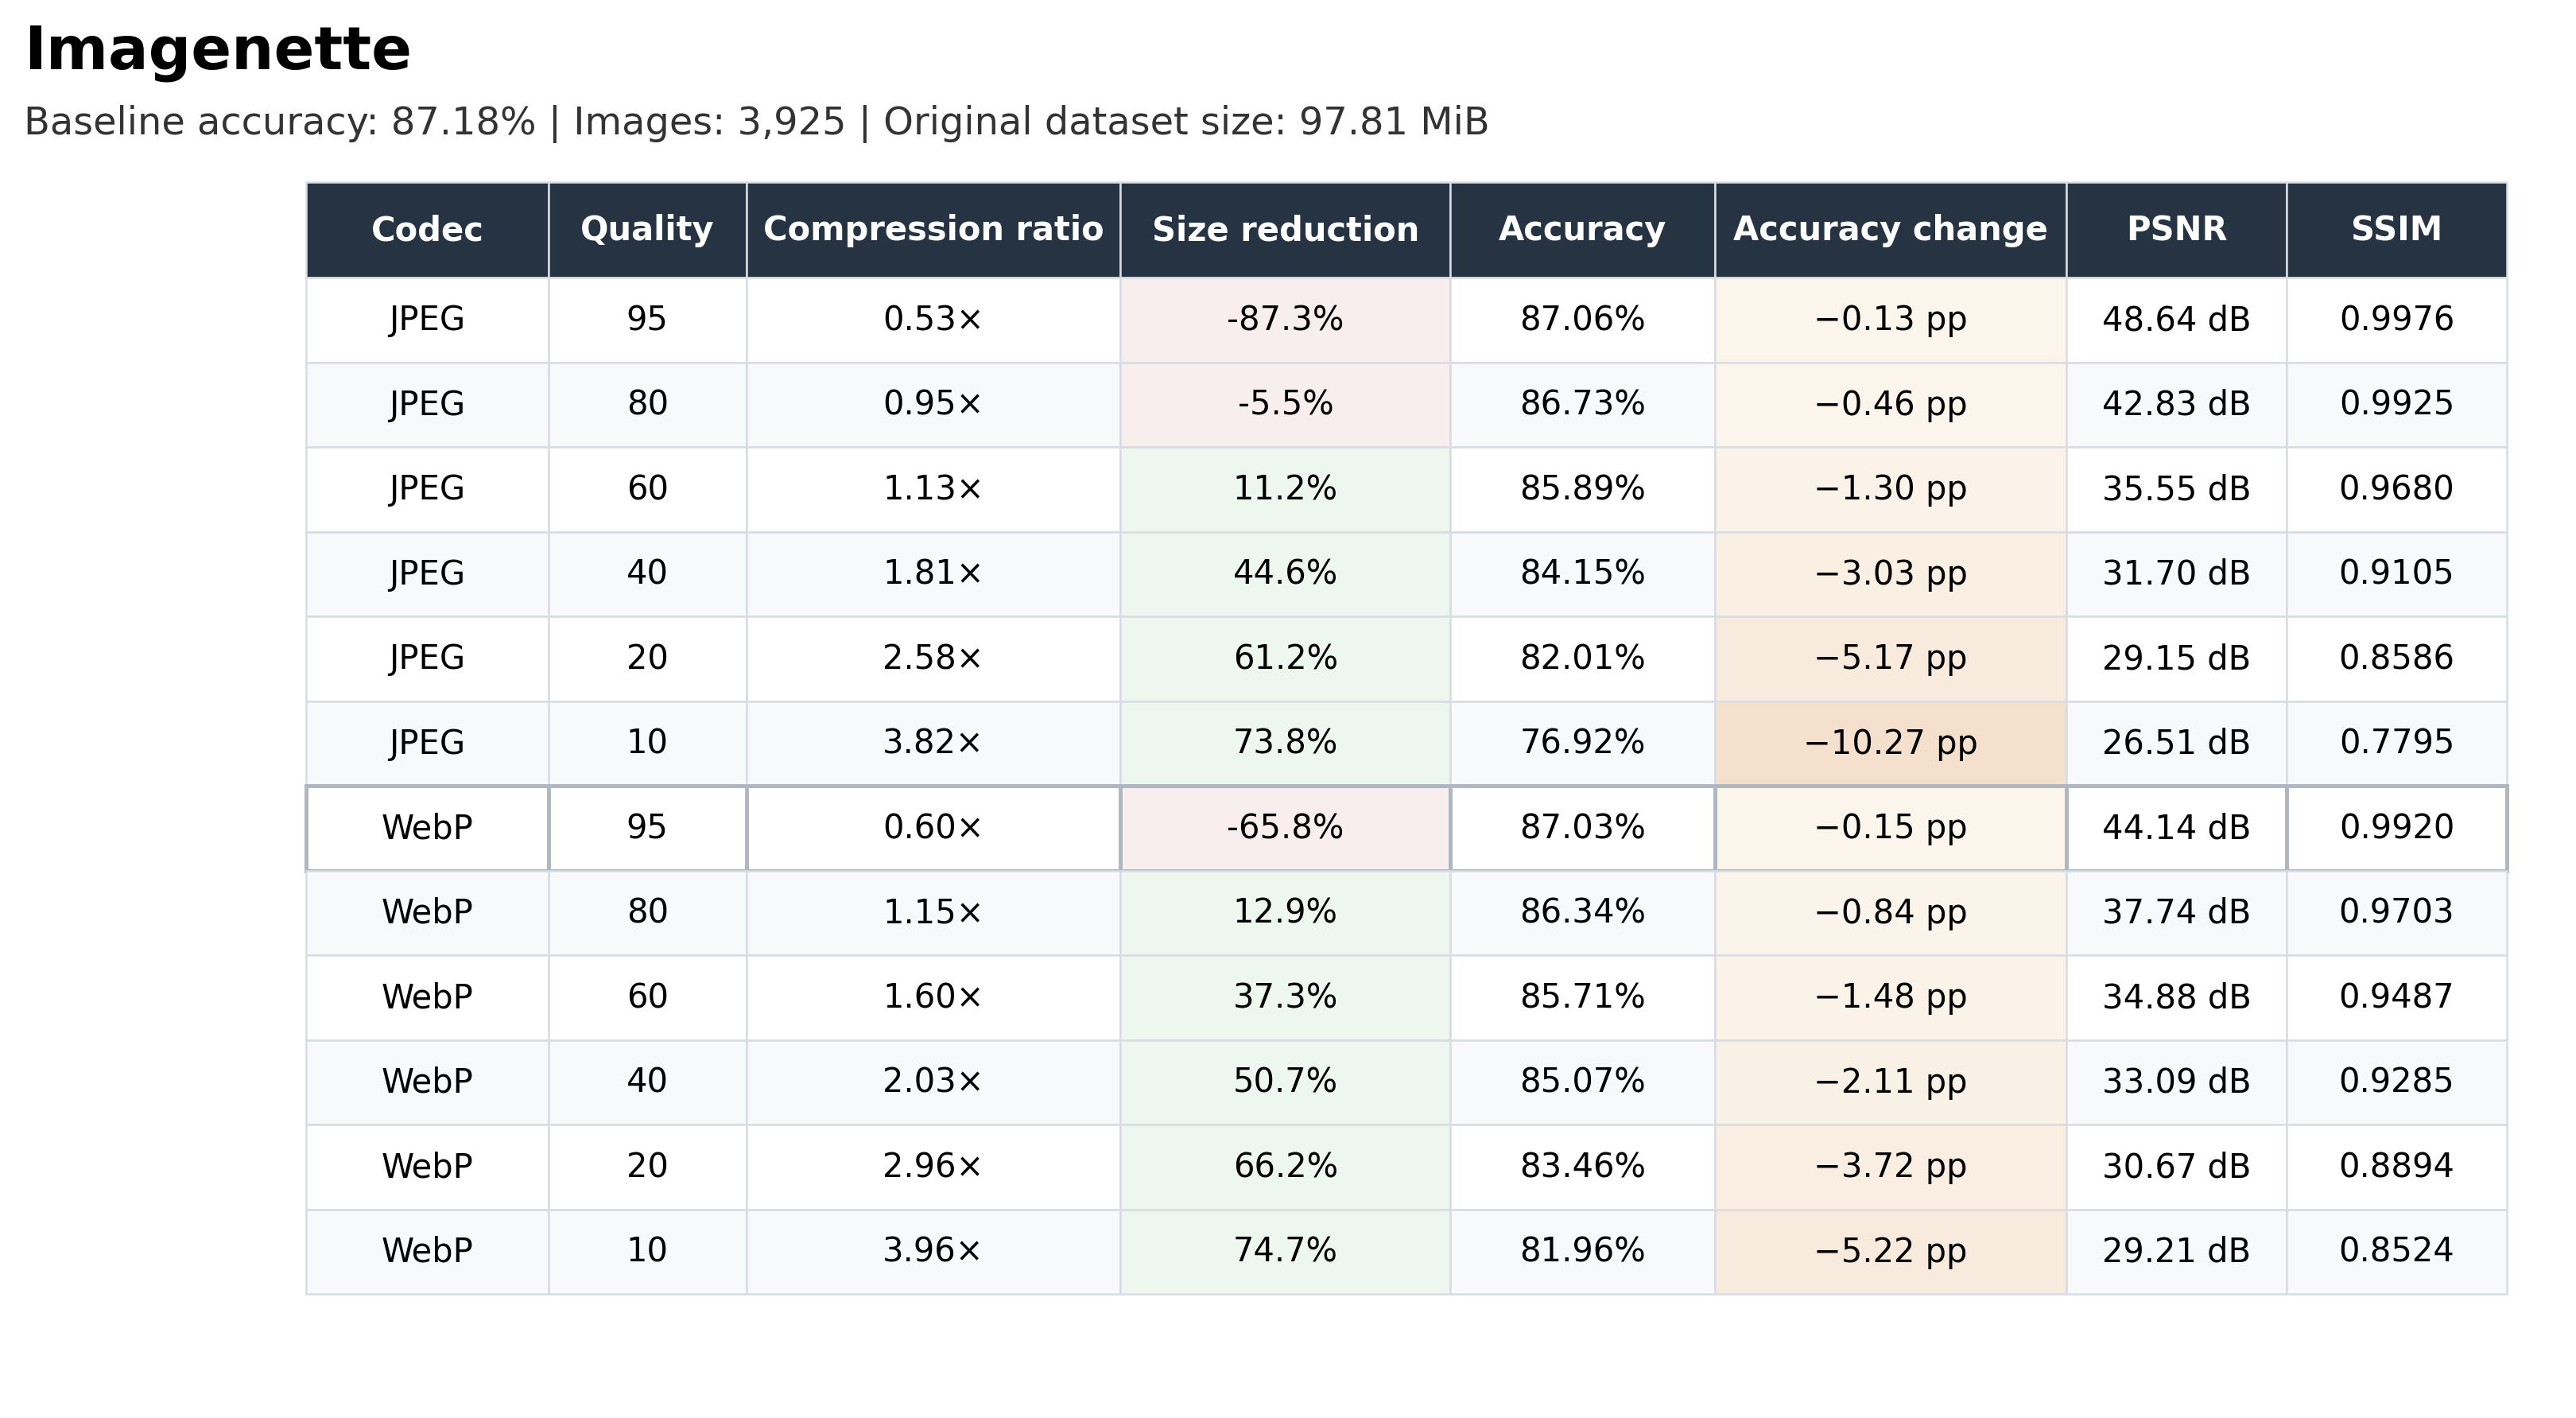
\includegraphics[width=0.90\textwidth]{../results/analysis/tables/imagenette_results_table.png}
    \caption{Imagenette aggregate rate--distortion--accuracy results for JPEG recompression and WebP transcoding.}
    \label{tab:imagenette-results}
\end{table}

\begin{table}[!htbp]
    \centering
    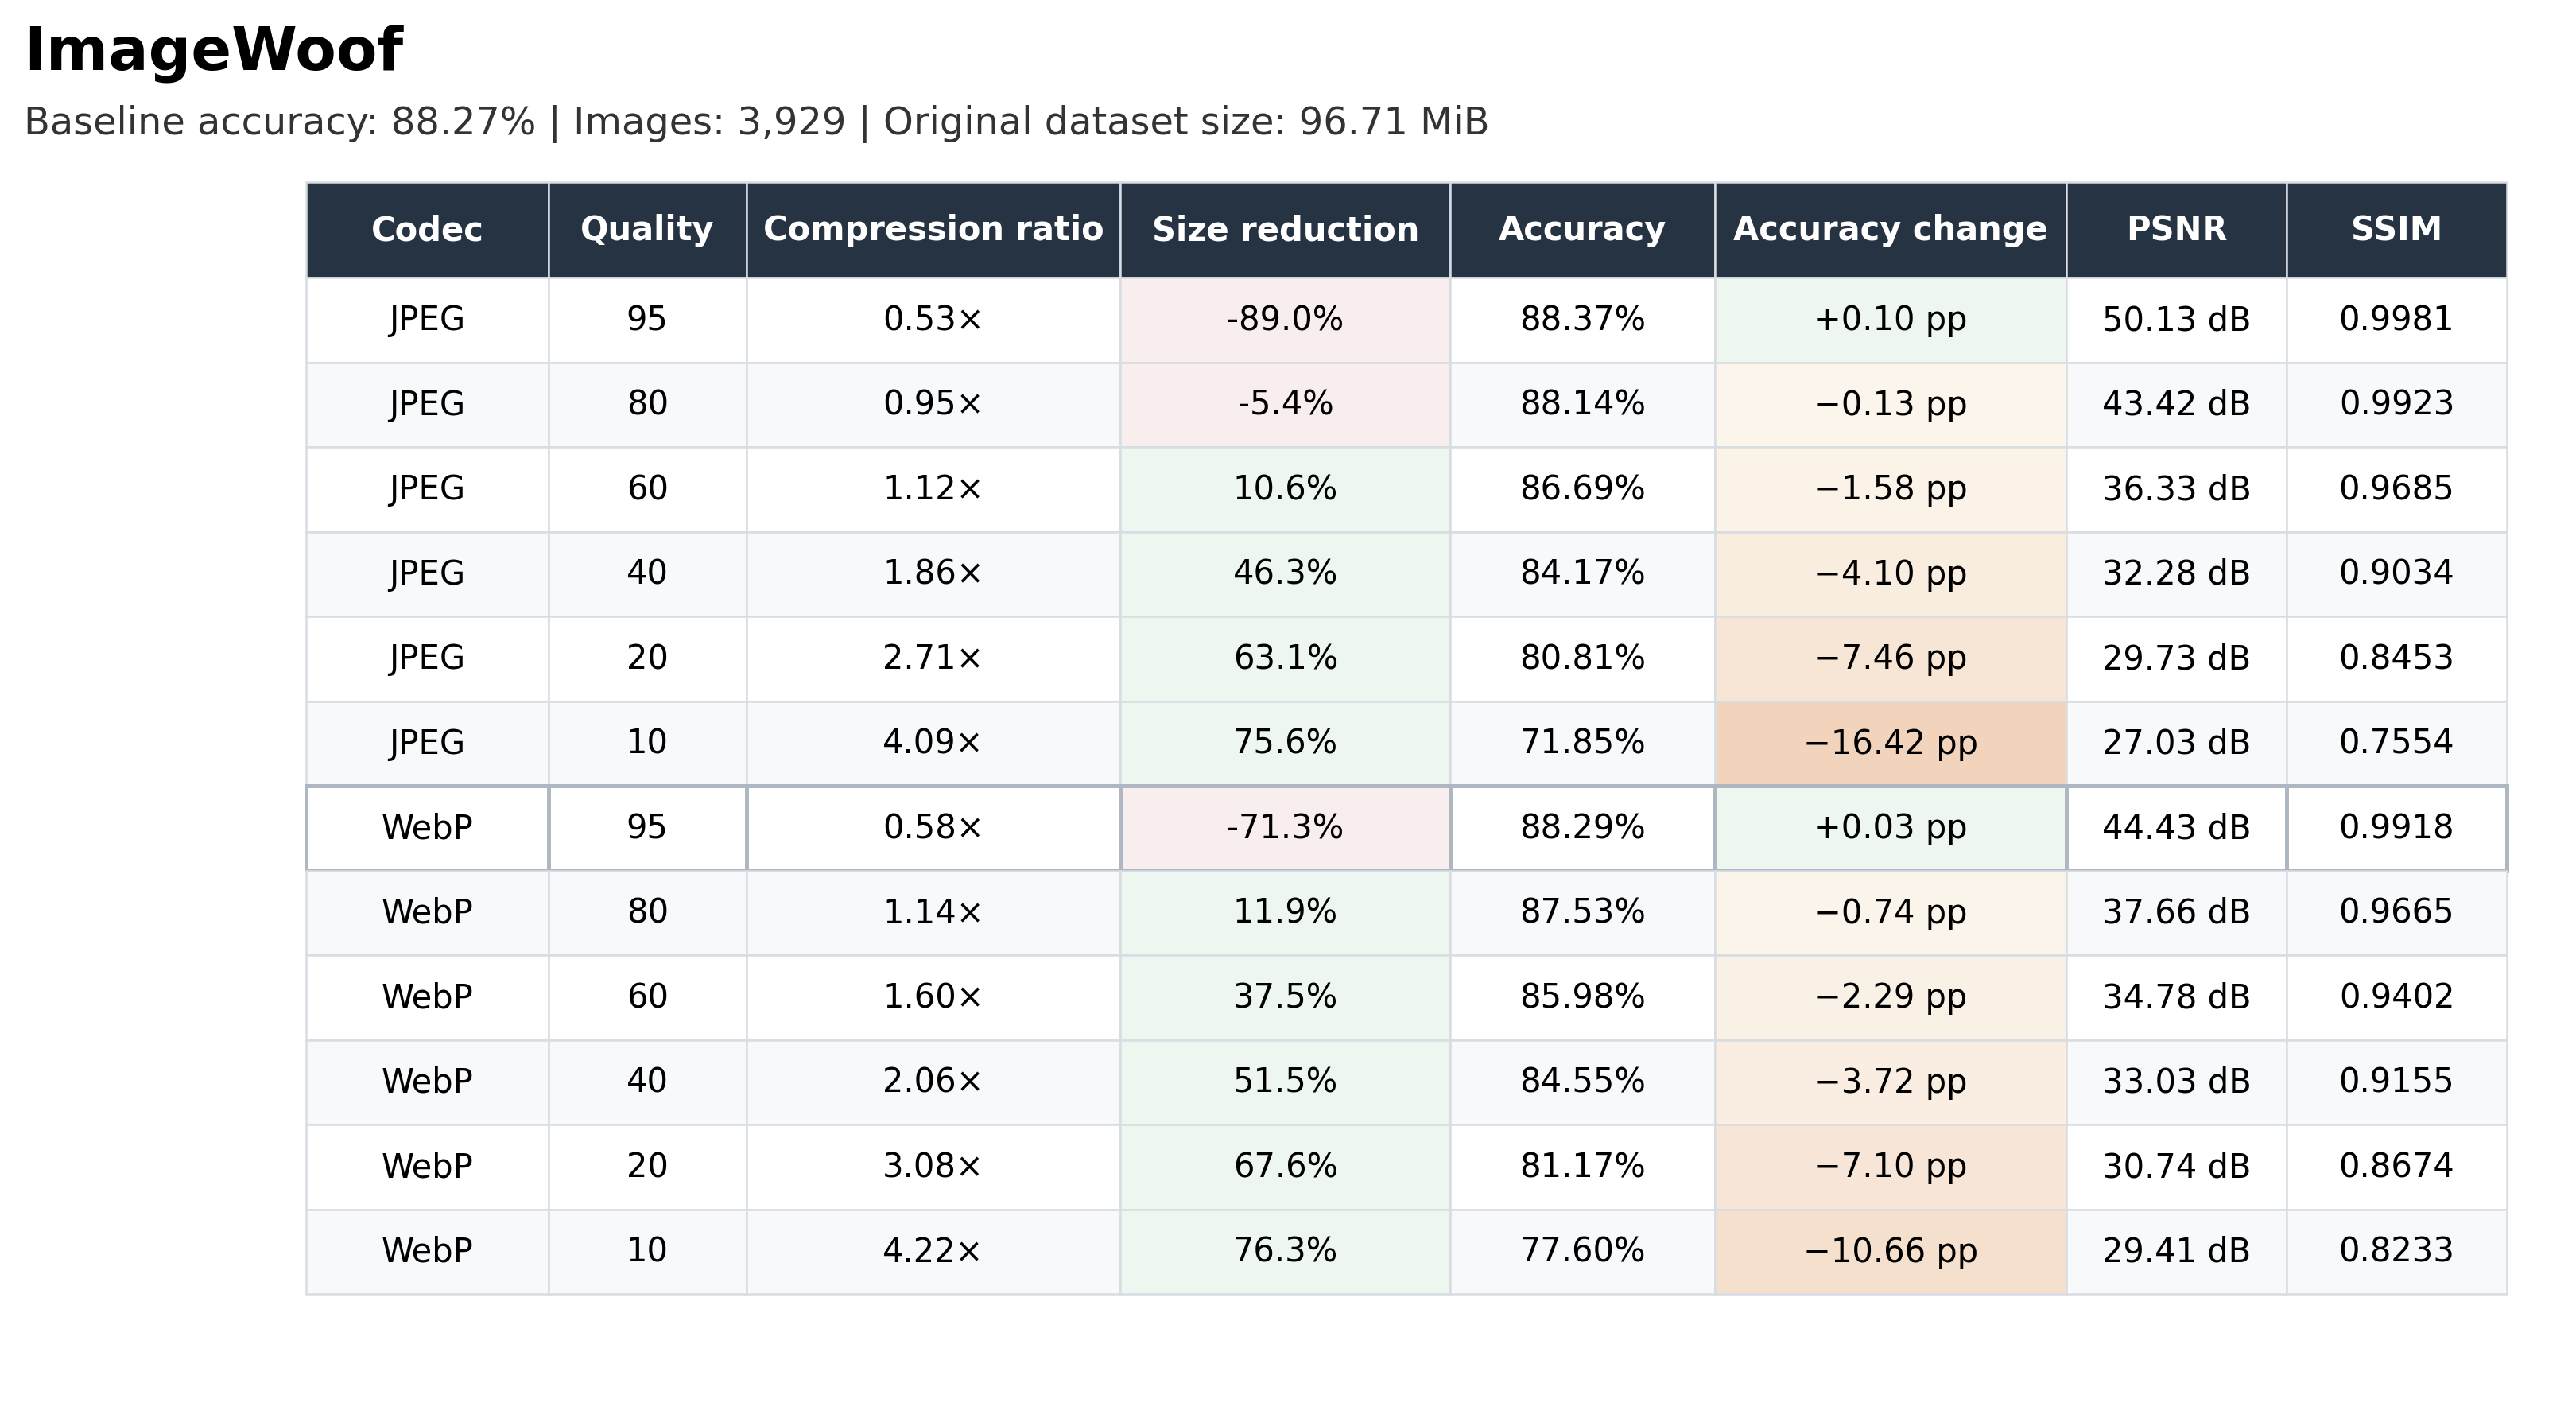
\includegraphics[width=0.90\textwidth]{../results/analysis/tables/imagewoof_results_table.png}
    \caption{ImageWoof aggregate rate--distortion--accuracy results for JPEG recompression and WebP transcoding.}
    \label{tab:imagewoof-results}
\end{table}

\FloatBarrier

\subsection{Rate--Accuracy Trade-off}

\begin{figure}[!htbp]
    \centering
    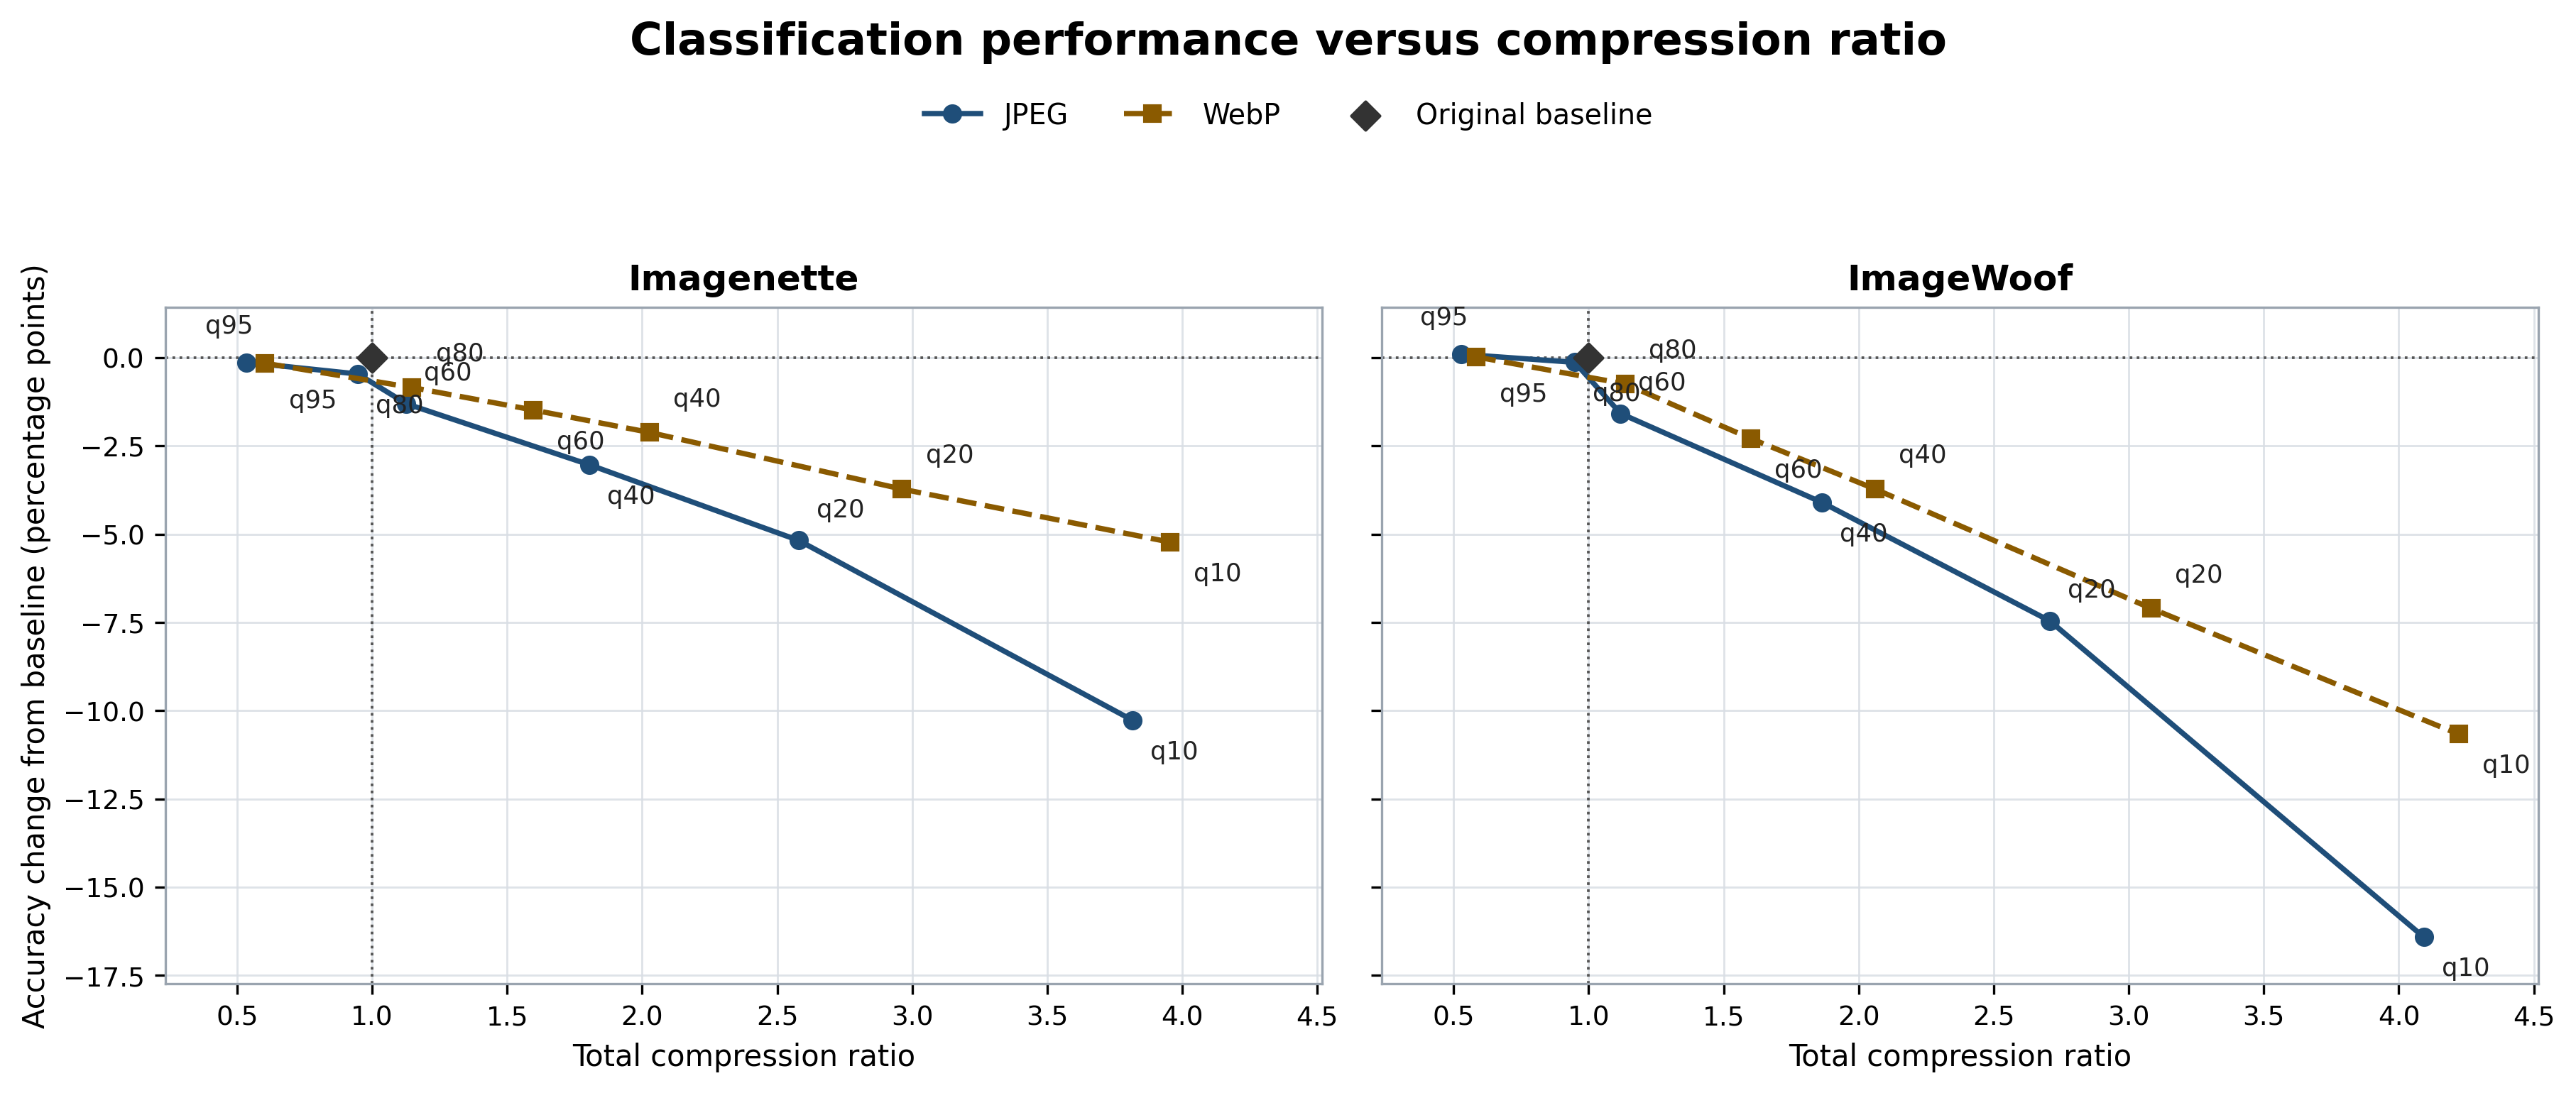
\includegraphics[width=0.92\textwidth]{../results/analysis/plots/rate_accuracy_tradeoff.png}
    \caption{Top-1 accuracy change relative to the original distributed JPEG baseline as a function of total compression ratio. Ratios below one indicate that recompression or transcoding increased the total file size.}
    \label{fig:rate_accuracy}
\end{figure}

Figure~\ref{fig:rate_accuracy} shows that conditions with compression ratios below 1 produce outputs larger than the source files. These conditions preserve accuracy close to the baseline but do not provide useful storage reduction. Once compression ratios exceed 1, greater compression is generally associated with larger classification losses, and the degradation becomes stronger at aggressive compression ratios. 

The first tested useful compression conditions are approximately JPEG q60 and WebP q80, where JPEG and WebP achieve comparable mild compression ratios. 

On Imagenette, JPEG q60 reaches a compression ratio of approximately 1.13 and changes accuracy by $-1.30$ percentage points, while WebP q80 reaches approximately 1.15 and changes accuracy by $-0.84$ percentage points. At these approximately matched rates, the observed WebP condition remains closer to the original classification accuracy. 

On ImageWoof, JPEG q60 reaches approximately 1.12 and changes accuracy by $-1.58$ percentage points, while WebP q80 reaches approximately 1.14 and changes accuracy by $-0.74$ percentage points. The difference between the two observed conditions is larger on ImageWoof. Aggressive JPEG recompression produces especially large losses on ImageWoof, but these comparisons are approximate because the compression ratios are close rather than exactly equal.

\clearpage

\subsection{Rate--Distortion Behaviour}

\begin{figure}[!htbp]
    \centering
    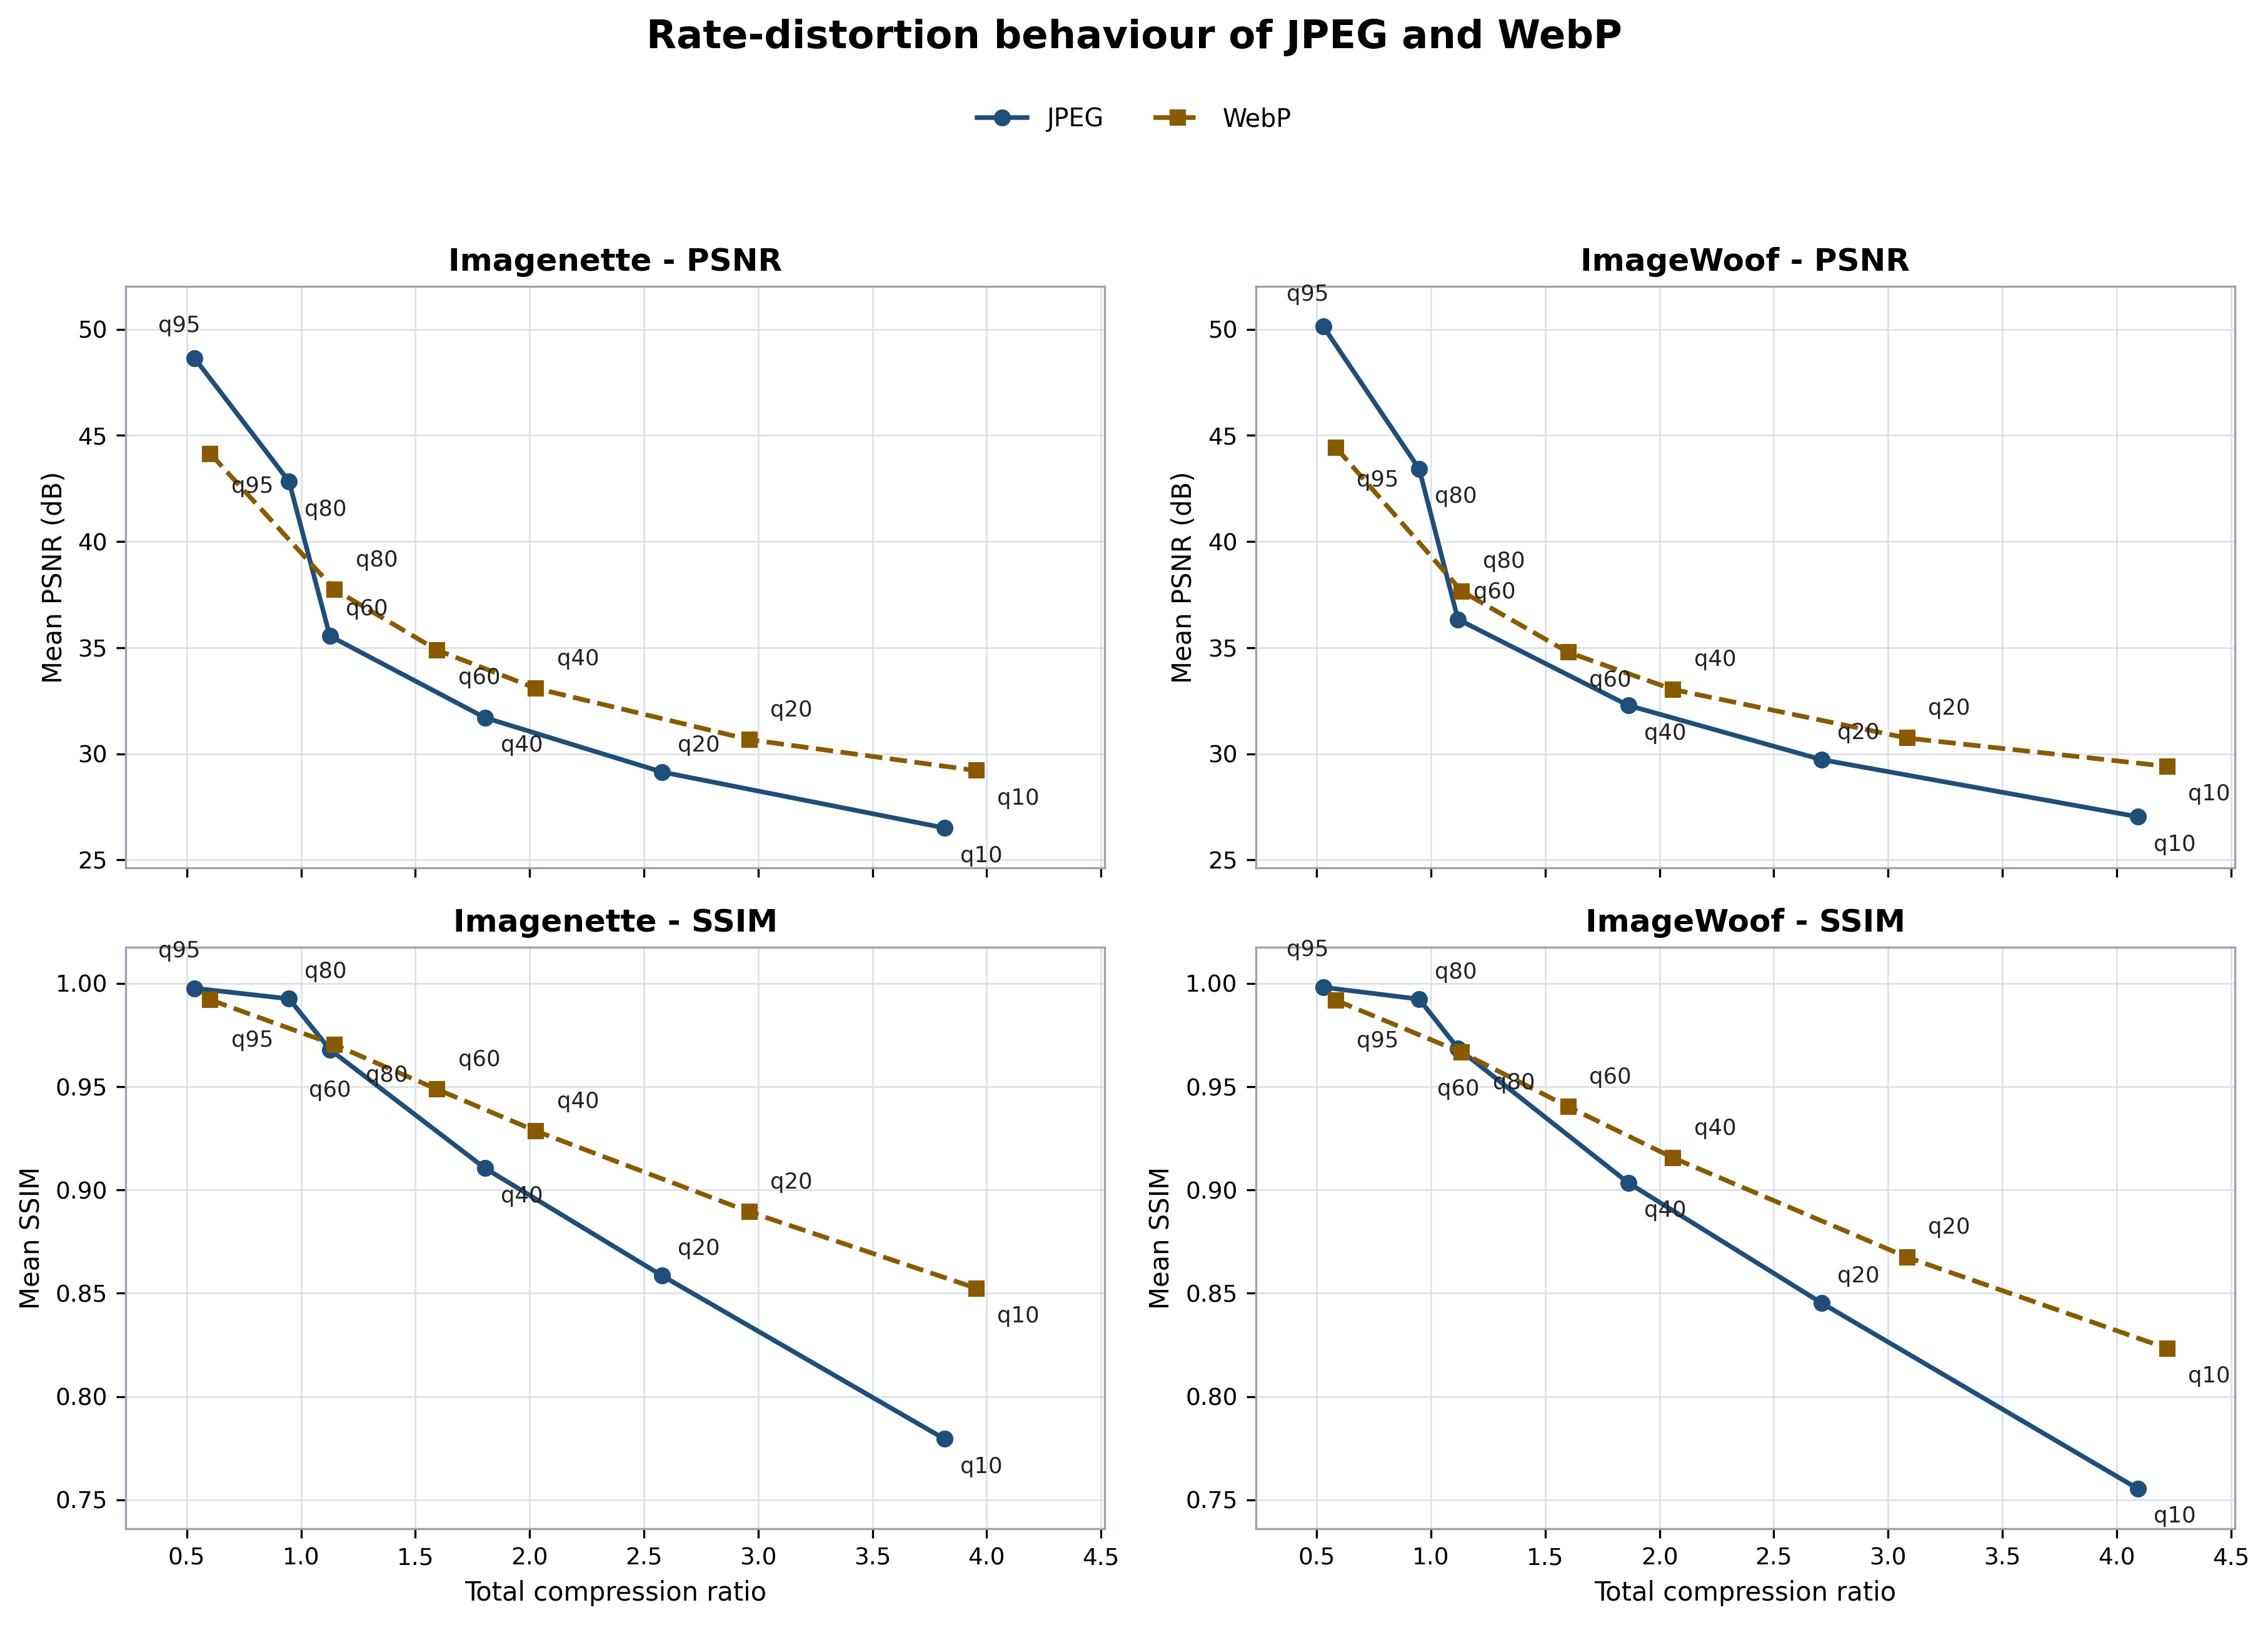
\includegraphics[width=0.82\textwidth]{../results/analysis/plots/rate_distortion_tradeoff.png}
    \caption{Mean PSNR and SSIM as functions of total compression ratio for JPEG recompression and WebP transcoding. Both metrics compare the decoded compressed image with the decoded distributed JPEG source image.}
    \label{fig:rate_distortion}
\end{figure}

\FloatBarrier

Figure~\ref{fig:rate_distortion} shows the expected rate--distortion relationship: mean PSNR decreases as compression becomes stronger, and mean SSIM also decreases as compression becomes stronger. This pattern appears for both datasets and both codecs. At stronger, approximately comparable compression ratios, the observed WebP curves generally retain higher mean PSNR and SSIM than JPEG, but this should not be interpreted as universal codec superiority. Considered together with Figure~\ref{fig:rate_accuracy}, the distortion results show why decoded image distortion and downstream classification performance should be evaluated jointly. For example, on ImageWoof, JPEG q60 has mean SSIM of approximately 0.9685 and an accuracy change of $-1.58$ percentage points, while WebP q80 has mean SSIM of approximately 0.9665 and an accuracy change of $-0.74$ percentage points. JPEG q60 therefore has a marginally higher mean SSIM in this comparison, but a larger classification loss. WebP q80 also has higher mean PSNR in the same comparison. This observation indicates that a higher aggregate SSIM does not necessarily imply better preservation of classifier performance. The spatial location and semantic relevance of the distortion may matter, but the current aggregate analysis does not directly test that mechanism.

\subsection{Targeted Threshold Refinement}

The exploratory analysis showed that the relevant accuracy-loss transition occurred in different quality regions for JPEG and WebP. This motivated the targeted evaluation of JPEG q70 and WebP q77 on both datasets. Both settings were evaluated to examine the region around the predefined 1 percentage-point tolerance. These quality values are codec-specific and should not be interpreted as equivalent settings.

\begin{table}[!htbp]
\centering
\small
\setlength{\tabcolsep}{3.5pt}
\resizebox{\textwidth}{!}{%
\begin{tabular}{lcrrrrrrl}
\toprule
Codec & Quality & Compression ratio & Size reduction & Accuracy & Accuracy loss & PSNR & SSIM & 1 pp \\
\midrule
JPEG & 70 & 1.03$\times$ & 3.2\% & 86.75\% & 0.43 pp & 41.50 dB & 0.9901 & Pass \\
WebP & 77 & 1.27$\times$ & 21.1\% & 86.06\% & 1.12 pp & 36.82 dB & 0.9645 & Fail \\
\bottomrule
\end{tabular}
}
\caption{Targeted refinement results for Imagenette.}
\label{tab:imagenette-refinement}
\end{table}

\begin{table}[!htbp]
\centering
\small
\setlength{\tabcolsep}{3.5pt}
\resizebox{\textwidth}{!}{%
\begin{tabular}{lcrrrrrrl}
\toprule
Codec & Quality & Compression ratio & Size reduction & Accuracy & Accuracy loss & PSNR & SSIM & 1 pp \\
\midrule
JPEG & 70 & 1.03$\times$ & 2.9\% & 87.55\% & 0.71 pp & 42.35 dB & 0.9913 & Pass \\
WebP & 77 & 1.26$\times$ & 20.5\% & 87.25\% & 1.02 pp & 36.72 dB & 0.9596 & Fail \\
\bottomrule
\end{tabular}
}
\caption{Targeted refinement results for ImageWoof.}
\label{tab:imagewoof-refinement}
\end{table}

\begin{figure}[!htbp]
    \centering
    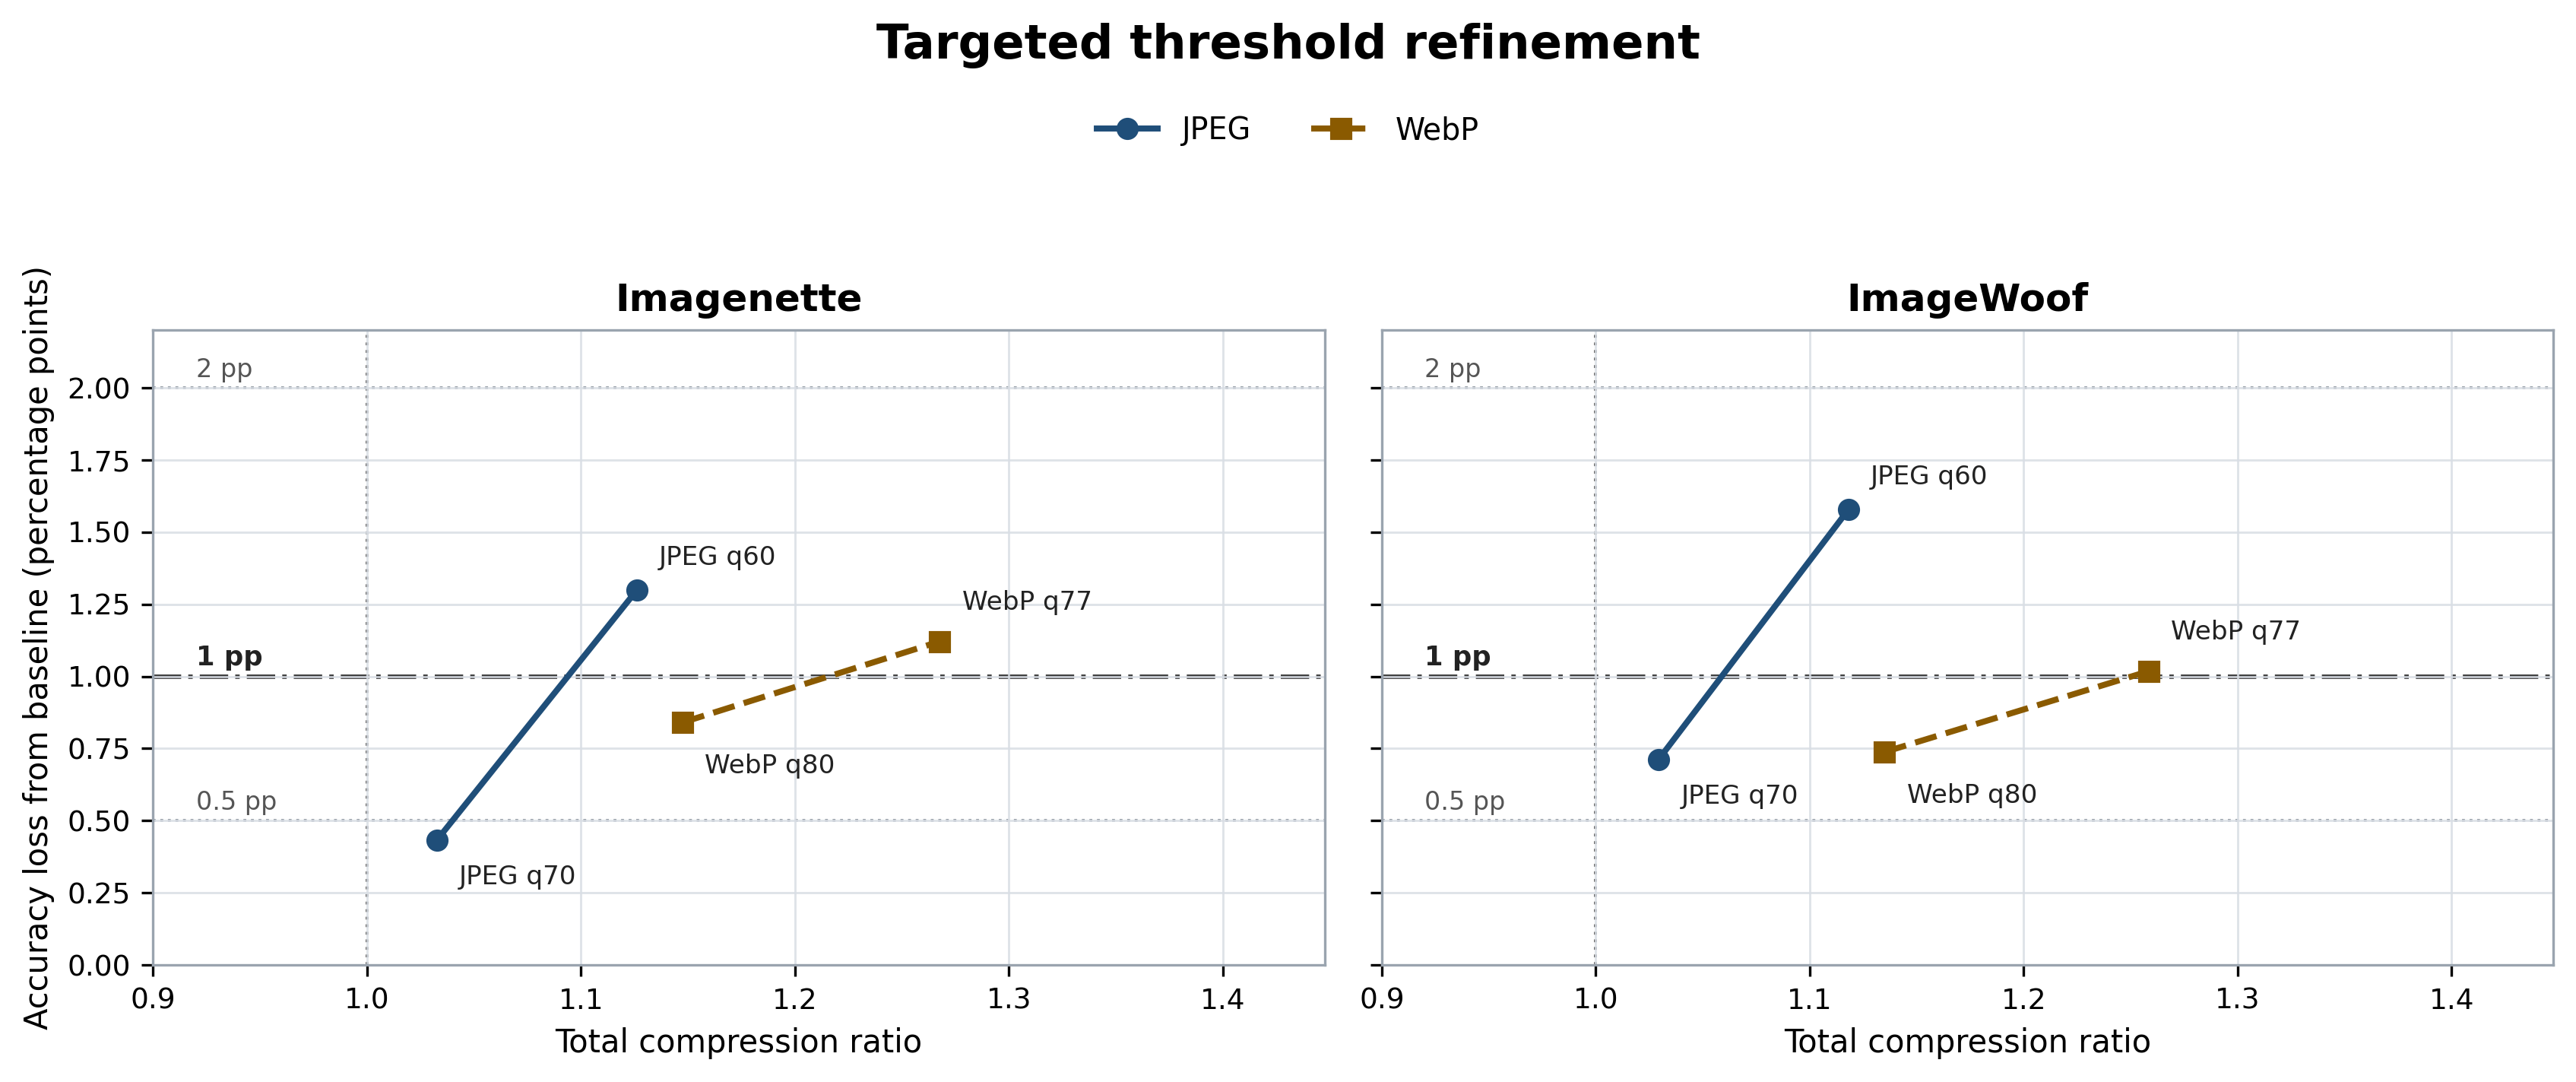
\includegraphics[width=0.87\textwidth]{../results/analysis/refinement/threshold_refinement.png}
    \caption{Targeted rate--accuracy refinement around the predefined tolerance region. JPEG q70 and WebP q77 are compared with the adjacent exploratory reference settings. The primary acceptable loss is 1 percentage point, with 0.5 and 2 percentage points shown as sensitivity margins.}
    \label{fig:threshold-refinement}
\end{figure}

Tables~\ref{tab:imagenette-refinement} and~\ref{tab:imagewoof-refinement}, together with Figure~\ref{fig:threshold-refinement}, show that JPEG q70 passes the primary tolerance on both datasets. It achieves high mean SSIM, approximately 0.99, and accuracy losses of 0.43 percentage points on Imagenette and 0.71 percentage points on ImageWoof. However, it reduces total size by only approximately 3\%. JPEG q60 provides greater storage reduction but exceeds the 1 percentage-point tolerance on both datasets. JPEG q70 is therefore the strongest tested JPEG condition satisfying the primary tolerance.

WebP q80 had already passed the primary tolerance on both datasets in the exploratory stage. WebP q77 was tested as a stronger compression point. It increases total size reduction to approximately 20--21\%, and mean SSIM remains relatively high, approximately 0.96. However, q77 slightly exceeds the primary tolerance, with an accuracy loss of 1.12 percentage points on Imagenette and 1.02 percentage points on ImageWoof. It must therefore be marked as failing the strict primary rule, while still being an informative near-boundary operating point. On ImageWoof, one changed prediction among 3,929 evaluated images corresponds to approximately 0.025 percentage points, so the difference between 1.00 and 1.02 percentage points is approximately at the resolution of one prediction. The fail designation is rule-based and should not be interpreted as evidence of a practically meaningful performance discontinuity at the 1 percentage-point boundary.

The observed points suggest that the candidate WebP operating interval lies between q80 and q77. WebP q80 reduces size by approximately 12--13\%, remains within the 1 percentage-point accuracy-loss tolerance, and retains SSIM close to 0.97. WebP q77 reduces size by approximately 20--21\%, retains SSIM close to 0.96, and exceeds the accuracy tolerance only slightly. The q77--q80 interval therefore defines a narrow and promising practical operating region. This interval offers a favourable trade-off between storage reduction, structural similarity, and classification preservation. An untested intermediate quality within this interval could plausibly provide a compromise between the two observed endpoints, but the exact operating point within this interval was not estimated because intermediate qualities were not evaluated.

\FloatBarrier

At the approximately matched storage reductions examined in this experiment, WebP obtains slightly greater storage reduction with lower classification loss. On Imagenette, JPEG q60 reduces size by 11.2\% with 1.30 percentage points loss, while WebP q80 reduces size by 12.9\% with 0.84 percentage points loss. On ImageWoof, JPEG q60 reduces size by 10.6\% with 1.58 percentage points loss, while WebP q80 reduces size by 11.9\% with 0.74 percentage points loss. Achieving a similar level of storage reduction through JPEG recompression required accepting a larger classification loss on both datasets. This is one of the principal codec-comparison findings of the study.
